% Source for the supplementary material to "Robust 3D gravity gradient inversion
% by planting anomalous densities" by Leonardo Uieda and Valeria C. F. Barbosa
\documentclass[twocolumn]{article}

% Packages for styling
\usepackage{graphicx} % For inserting figures
\usepackage{amssymb,amsmath} % Mathematical Symbols and fonts
\usepackage{natbib} % For pretty references
\usepackage[a4paper]{geometry} % To set the margins
\geometry{verbose,tmargin=2cm,bmargin=2cm,lmargin=1.5cm,rmargin=1.5cm}

% For pdf hyperlinks
\usepackage[pdftex]{hyperref}
\hypersetup{colorlinks=true}
\hypersetup{citecolor=blue}
\hypersetup{urlcolor=blue}
\hypersetup{pdftitle={Supplementary material to
    "Robust 3D gravity gradient inversion by planting anomalous densities"
    by Leonardo Uieda and Valeria C. F. Barbosa}}
\hypersetup{pdfauthor={Leonardo Uieda and Valeria C. F. Barbosa}}
\usepackage{url}

% Custom math commands
\newcommand{\vect}[1]{\mathbf{#1}}
\newcommand{\mat}[1]{\mathbf{#1}}
\newcommand{\comp}[1]{#1^{\alpha\beta}}
\newcommand{\norm}[1]{\left|\left|#1\right|\right|}

\begin{document}

% The title and authors
\title{\textbf{\Large
Supplementary material to\\[0.15cm]
``Robust 3D gravity gradient inversion by planting anomalous densities''\\
by Leonardo Uieda and Val\'eria C. F. Barbosa}\footnote{Submitted to journal
\textit{GEOPHYSICS} on October 3, 2011.}}
\author{Leonardo Uieda$^{1}$ and Val\'eria C. F. Barbosa$^{2}$\\[0.2cm]
    {\small
    Observat\'orio Nacional, Rio de Janeiro, Brazil.
    Contact e-mail: 
    $^{1}$ \href{mailto:leouieda@gmail.com}{leouieda@gmail.com}~;
    $^{2}$ \href{mailto:valcris@on.br}{valcris@on.br}}}

\maketitle

\section*{\normalsize\center ABSTRACT}
We provide supplementary material to
``Robust 3D gravity gradient inversion by planting anomalous densities''
by Leonardo Uieda and Val\'eria C. F. Barbosa.
The material included are:
(1) plots of the predicted and synthetic $g_{yy}$ and $g_{yz}$ components
from the section ``Application to synthetic data'',
(2) plots of the results of the sensitivity analysis to
uncertainties in the density-contrast value of the seeds,
(3) the contour maps of the synthetic and predicted data
for the synthetic tests in the ``Sensitivity analysis'' section,
and
(4) a synthetic test illustrating the use of
the $\ell_{2}$-norm of the residual vector
in the data-misfit function.


\vspace{-0.7cm}
\section*{\normalsize\center MISSING FIGURES FROM ``APPLICATION TO SYNTHETIC DATA''}

Figure~\ref{fig:synth-fit} shows
the synthetic (color-scale maps) and predicted (black contour lines) data of the
$g_{yy}$ and $g_{yz}$ components of the gravity gradient tensor.
The synthetic data were produced
by multiple targeted and non-targeted sources
shown in Figure 5a of Uieda and Barbosa (2012).
The predicted data were produced by
the inversion result shown in
Figure 5c of Uieda and Barbosa (2012).

\begin{figure}[]
    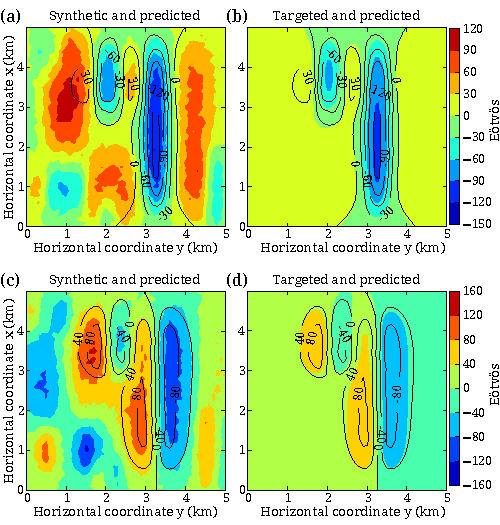
\includegraphics{fig/synthetic-fit-gyy-gyz}
    \caption{  
    Test with synthetic data 
    produced by multiple targeted and non-targeted sources
    shown in Figure 5a of Uieda and Barbosa (2012).
    (a) Synthetic noise-corrupted data (color-scale map)
    of the $g_{yy}$ component of the gravity gradient tensor
    produced by targeted and non-targeted sources. 
    (b) Synthetic data (color-scale map)
    of the $g_{yy}$ component
    produced by the targeted sources only.
    (c) Synthetic noise-corrupted data (color-scale map)
    of the $g_{yz}$ component of the gravity gradient tensor
    produced by targeted and non-targeted sources. 
    (d) Synthetic data (color-scale map)
    of the $g_{yz}$ component
    produced by the targeted sources only.
    In a-d the predicted data (black contour lines) are
    produced by the inversion result
    shown in Figure 5c of Uieda and Barbosa (2012).
    \label{fig:synth-fit}}
\end{figure}

\vspace{-0.7cm}
\section*{\normalsize\center MISSING FIGURES FROM ``SENSITIVITY ANALYSIS''}

Here, we provide additional figures
for the section ``Sensitivity analysis''
of Uieda and Barbosa (2012).
Figure~\ref{fig:sensanal-under} shows
the results obtained by using correct seed locations
but a density contrast lower than the true one.
The estimated density-contrast distribution
(light gray prisms in Figure~\ref{fig:sensanal-under})
has a larger volume than the true source
(black outlines in Figure~\ref{fig:sensanal-under}).
\\
\indent
Figure~\ref{fig:sensanal-over} shows
the results obtained by using correct seed locations
but a density contrast larger than the true one.
The estimated density-contrast distribution
(dark gray prisms in Figure~\ref{fig:sensanal-over})
has a smaller volume than the true source
(black outlines in Figure~\ref{fig:sensanal-over}).
\\
\indent
Figure~\ref{fig:sensanal-fit} shows
the synthetic (color-scale maps) and
predicted (black contour lines) data
of the $g_{zz}$ component of the gravity gradient tensor
for all tests in the ``Sensitivity analysis'' section
of Uieda and Barbosa (2012).

\begin{figure}[]
    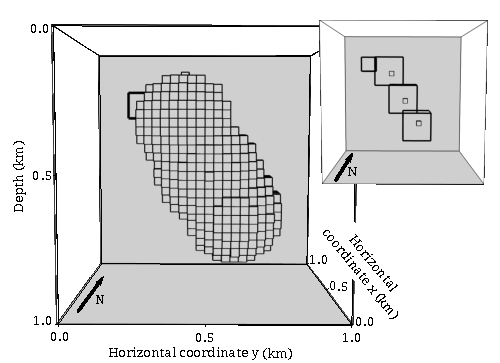
\includegraphics{fig/sensitivity-under}
    \caption{     
    Analysis of the sensitivity to uncertainties in the location of the seeds.
    Test using ideal seed locations
    but a density contrast of $0.3\ \mathrm{g/cm}^3$,
    which is smaller than the true one ($1.0\ \mathrm{g/cm}^3$).
    The outline of the true sources are shown in solid black lines.
    The inversion result is shown as light gray prisms.
    Prisms with zero density contrast are not shown.
    The inset shows the three seeds used in the inversion (light gray prisms)
    and the outline of the true sources (solid black lines).
    The location of the seeds was chosen
    in order to outline the correct dip of
    the large dipping source (targeted source).
    \label{fig:sensanal-under}}
\end{figure}
\begin{figure}[]
    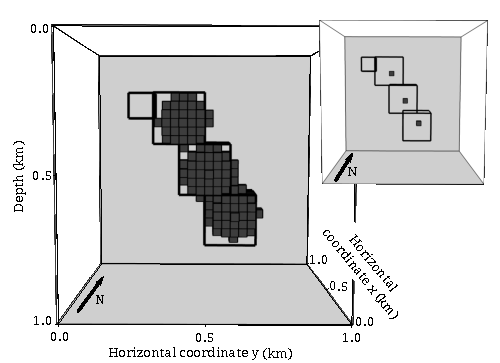
\includegraphics{fig/sensitivity-over}
    \caption{      
    Analysis of the sensitivity to uncertainties in the location of the seeds.
    Test using ideal seed locations
    but a density contrast of $1.5\ \mathrm{g/cm}^3$,
    which is larger than the true one ($1.0\ \mathrm{g/cm}^3$).
    The outline of the true sources are shown in solid black lines.
    The inversion result is shown as dark gray prisms.
    Prisms with zero density contrast are not shown.
    The inset shows the three seeds used in the inversion (dark gray prisms)
    and the outline of the true sources (solid black lines).
    The location of the seeds was chosen
    in order to outline the correct dip of
    the large dipping source (targeted source).
    \label{fig:sensanal-over}}
\end{figure}
\begin{figure}[]
    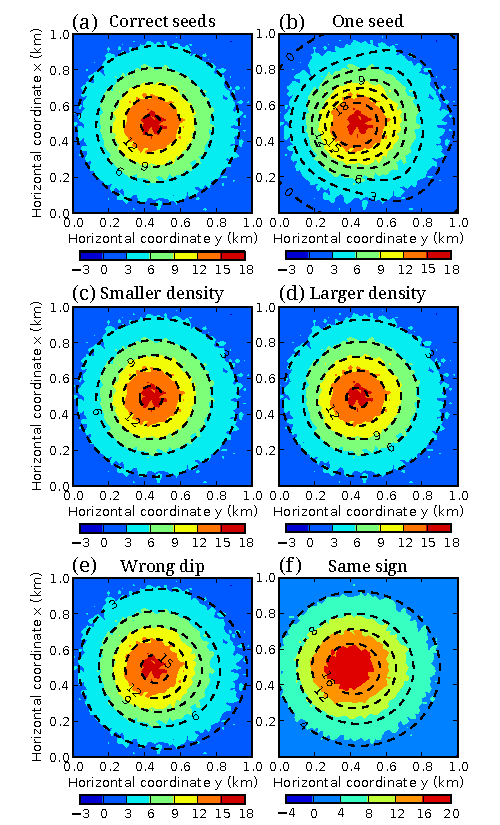
\includegraphics{fig/sensitivity-fit}
    \caption{      
    Sensitivity analysis of the method of planting anomalous densities.
    The synthetic (color-scale maps) and
    predicted (black contour lines) data
    of the $g_{zz}$ component
    for all tests.
    (a) The test with correct seed locations and density contrasts
        (see Figure 6 of Uieda and Barbosa, 2012).
    (b) The test with only a single seed
        located at the top of the large dipping source (targeted source)
        (see Figure 8 of Uieda and Barbosa, 2012).
    (c) The test with correct seed locations
        but a density contrast lower than the true one
        (Figure~\ref{fig:sensanal-under}).
    (d) The test with correct seed locations
        but a density contrast larger than the true one
        (Figure~\ref{fig:sensanal-over}).
    (e) The test with seeds
        that follow an incorrect dip of
        the large dipping source (targeted source)
        (see Figure 7 of Uieda and Barbosa, 2012).
    (f) The test with correct seed locations and density contrasts,
        but with a non-targeted source with a density contrast
        of the same sign as that of the targeted source
        (see Figure 9 of Uieda and Barbosa, 2012).
    Color-scale units are E\"otv\"os.
    \label{fig:sensanal-fit}}
\end{figure}

\vspace{-0.7cm}
\section*{\normalsize\center APPLICATION TO SYNTHETIC DATA USING THE~$\ell_{2}$-NORM}

Figure~\ref{fig:synthl2-fit} shows
a set of color-scale maps of the synthetic noise-corrupted
$g_{xx}$, $g_{xy}$, $g_{xz}$, $g_{yy}$, $g_{yz}$, and $g_{zz}$ components
of the gravity gradient tensor
calculated at 150 meter height.
The data were contaminated with pseudorandom Gaussian noise
with zero mean and 5 E\"otv\"os standard deviation.
Each tensor component was calculated on a regular grid
of $26\times 26$ observation points in the $x$- and $y$-directions,
totaling a data set of 4,056 observations,
with a grid spacing of 0.2 km along both directions.
The synthetic data were produced by four closely separated sources
(Figure~\ref{fig:synthl2-res}a).
These sources are rectangular parallelepipeds
with different sizes and depths and with density contrasts
ranging from $-1\ \mathrm{g/cm}^{3}$ to $1\ \mathrm{g/cm}^{3}$.
In this test, all four sources are considered targets of the interpretation.
\\
\indent
Because we did not consider the presence of geologic noise
(non-targeted sources),
the inversion was performed using
the normalized $\ell_{2}$-norm of the residual vector,
instead of the $\ell_{1}$-norm,
in the data misfit function, i.e.,

\begin{equation}
\phi_{\alpha\beta}(\vect{p}) =
\dfrac{\norm{\vect{r}^{\alpha\beta}}_2}{\norm{\vect{g}^{\alpha\beta}}_2} =
\sqrt{
    \dfrac{\sum\limits_{i=1}^{L}\left(g_i^{\alpha\beta} -
        d_i^{\thinspace\alpha\beta}\right)^{2}}
    {\sum\limits_{i=1}^{L}\left(g_i^{\alpha\beta}\right)^{2}}.}
\end{equation}


We assigned a total of 18 seeds (Figure~\ref{fig:synthl2-res}b)
distributed between the four sources as follows:
seven for the source with density contrast of $1\ \mathrm{g/cm}^{3}$ (in red);
five for source with density contrast of $-1\ \mathrm{g/cm}^{3}$ (in blue);
four for the source with density contrast of $0.7\ \mathrm{g/cm}^{3}$ (in yellow);
two for the source with density contrast of $0.9\ \mathrm{g/cm}^{3}$ (in orange).
We used an interpretative model
consisting of 25,000 juxtaposed right rectangular prisms.
The inversion control variables were
$\mu = 0.1$ and $\delta = 0.0001$.
The inversion result in Figure~\ref{fig:synthl2-res}c
shows that our method estimates a density-contrast distribution
composed of four compact sources
(i.e., without hollows)
whose shapes very closely resemble
the shape of the four true sources (Figure~\ref{fig:synthl2-res}a),
regardless of their depth, size, or density contrast.
This estimated density-contrast distribution
produces predicted data that fit the observed data
as shown in Figure~\ref{fig:synthl2-fit}.

\begin{figure}[]
    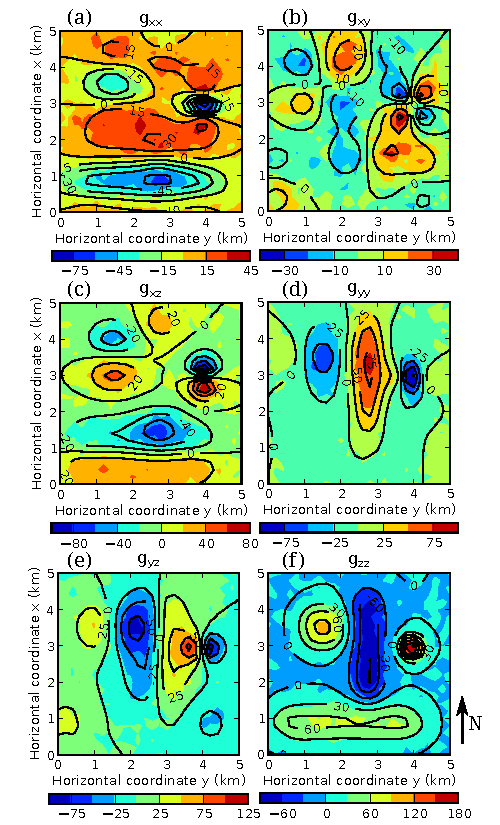
\includegraphics{fig/synthetic-l2-fit}
    \caption{
        Test with synthetic data produced by multiple targeted sources
        and using the $\ell_{2}$-norm of the residual vector.
        Synthetic noise-corrupted data (color-scale maps) and
        data predicted by the inversion result (black contour lines)
        of the (a) $g_{xx}$, (b) $g_{xy}$, (c) $g_{xz}$, (d) $g_{yy}$, (e) $g_{yz}$, and (f) $g_{zz}$
        components of the gravity gradient tensor.
        The synthetic data are produced by
        the four prisms shown in Figure~\ref{fig:synthl2-res}a.
        The predicted is produced by
        the estimated density-contrast distribution
        shown in Figure~\ref{fig:synthl2-res}c.
        Color-scale units are E\"otv\"os.
    \label{fig:synthl2-fit}}
\end{figure}
\begin{figure}[]
    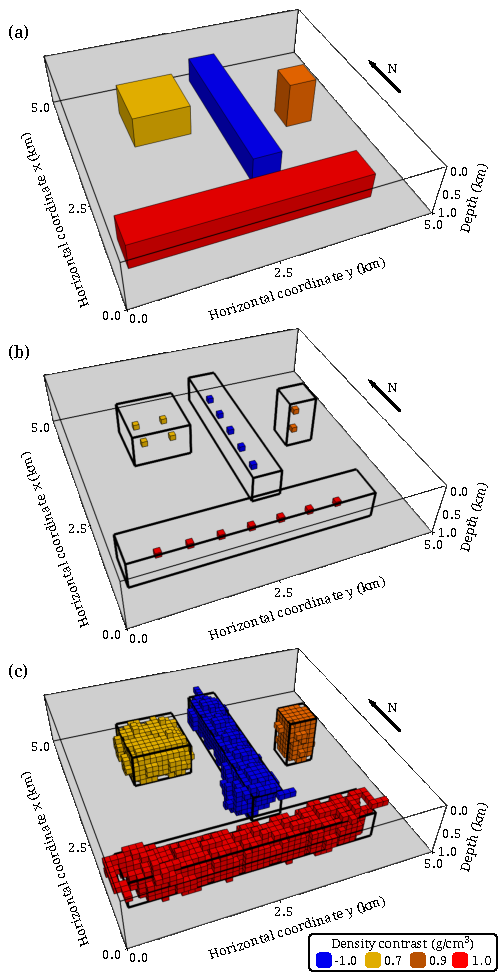
\includegraphics{fig/synthetic-l2-result}
    \caption{
        Test with synthetic data produced by multiple targeted sources and
        using the $\ell_{2}$-norm of the residual vector.
        (a) Perspective view of the four targeted sources
        used to generate the synthetic data
        shown in Figure~\ref{fig:synthl2-fit}.
        (b) The 18 seeds used in the inversion. 
        (c) Inversion result using the $\ell_{2}$-norm of the residual vector.
        Prisms of the interpretative model
        with zero density contrast are not shown.
        Black lines represent the frame of the true targeted sources.
    \label{fig:synthl2-res}}
\end{figure}



\end{document}
